% Last updated: 2023/02/19 20:40:17
\documentclass[9pt,twocolumn]{jsarticle}
\usepackage{klresume}
\usepackage{amsmath}
\begin{document}

\type{B} %卒論はB,修論はM
\term{F} %中間審査はM,最終審査はF
\author{須崎 良祐}
\id{27020729} %学籍番号
\fyear{2023} %修了・卒業年度(修了・卒業式が2024年3月なら2023年度)
\title{飲食店推薦のための機械学習アルゴリズムの比較}
\maketitle

\section{はじめに}
近年では推薦システムの研究は盛んに行われているが,そのうちの1つに,決定木を用いた音楽推薦システムの研究\cite{c}がある.
この研究では,決定木と他の機械学習アルゴリズムを比較して,決定木の有効性を示している. 
この研究では,音楽データを扱った音楽推薦における場合で決定木の有効性を示しているが,飲食店データを扱った飲食店推薦における場合でも決定木の有効性を明確にする必要がある. 
本研究では,木構造を使った決定木と線形モデルであるロジスティック回帰,非線形モデルであるk-NNを比較し,飲食店推薦における決定木の有効性を明確化することを目的とする.

\section{決定木を用いた飲食店推薦}
\subsection{推薦に用いる飲食店データと特徴量}
本研究で扱う推薦に用いる飲食店データは,ジャンル(13種類),個室の有無,喫煙席の有無,Wi-Fiの有無,駐車場の有無,価格帯,総合評価である.
これらを0か1といった離散値,0から1にスケーリングされた連続値に変換し,特徴量として扱う.

\subsection{決定木}
図\ref{fig10}のように,データセット(複数の飲食店データと,それらに対する評価)から作成された木構造である.
根は,データセット全体を含んでおり,データの特徴に基づいて最初の分割条件が決められる場所である.
図\ref{fig10}において,根から分割する条件は「喫煙席の有無」であったため,喫煙席がある飲食店を左の子,喫煙席が無い飲食店を右の子に分岐する.
左の子は,「行きたくない」飲食店のみが格納されているため,これ以上分岐させる必要が無くなり,葉となる.
右の子は,「行きたくない」飲食店も「行きたい」飲食店も格納されているため,まだ分岐させる必要がある.
右の子から分割する条件は「駐車場の有無」であったため,駐車場がある飲食店を左の孫,駐車場が無い飲食店を右の孫に分岐する.
右の2つの孫は,「行きたい」あるいは「行きたくない」どちらかの飲食店のみが格納されているため,これ以上分岐させる必要が無くなり,葉となる.
このような決定木を元に,未知の飲食店データに対する評価の予測を行う,
\begin{figure}[htbp]
    \begin{center}
      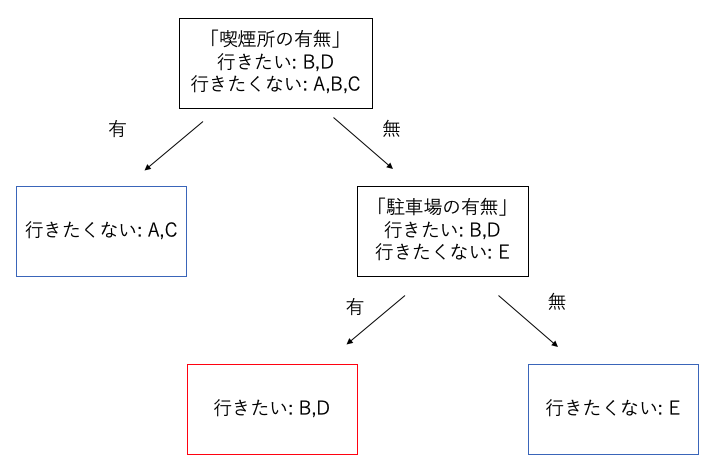
\includegraphics[width=6cm]{image/fig10.png}
      \caption{得られた決定木}
      \label{fig10}
    \end{center}
\end{figure}

\subsection{ロジスティック回帰}
ロジスティック回帰は,飲食店データとそれらに対する評価を使って,特徴量に対する重みを学習し,その重みと未知の飲食店の特徴量から,未知の評価飲食店データの予測を行う手法である.
その予測は,未知の飲食店に対して「行きたい」と評価する確率\(\hat{p}\)で決まる.
\[
\sigma(t) = \frac{1}{1 + e^{-t}}
\]
\[
\hat{p} = \sigma\left(\sum_{i=1}^{19} w_i x_i\right)
\]

\( t \)は飲食店の各特徴量と各特徴量に対する重みの積の総和,
\( \sigma(t) \)は入力値\( t \)のシグモイド関数,\( x_i \)は\( i \)番目の特徴量(ジャンル13種類と,その他6つの特徴量),\( w_i \)は\( i \)番目の特徴量に対する重みである.
つまり,\(\hat{p}\)が0.5を越えていれば「行きたい」と予測し,0.5以下であれば「行きたくない」と予測する.

\subsection{k-NN}
k-NNは,未知の飲食店データから,最も特徴ベクトル間の距離が近い\( k \)個の飲食店データの評価の多数決で,未知の飲食店データの評価の予測を行う手法である.
\section{評価}

\subsection{比較の結果}
飲食店データ100件と,それらに対する3人の評価を使って,各アルゴリズムで10フォールド交差検証を行ったところ,それぞれのアルゴリズムの平均精度は図\ref{fig7}のようになり,決定木が最も良かった.

また,最も精度が良かった決定木と他のアルゴリズムの精度間に,有意水準5%で統計的な有意差が存在するかどうかを調べるために,ウィルコクソンの符号順位検を行った結果も示している.

\begin{figure}[htbp]
    \begin{center}
      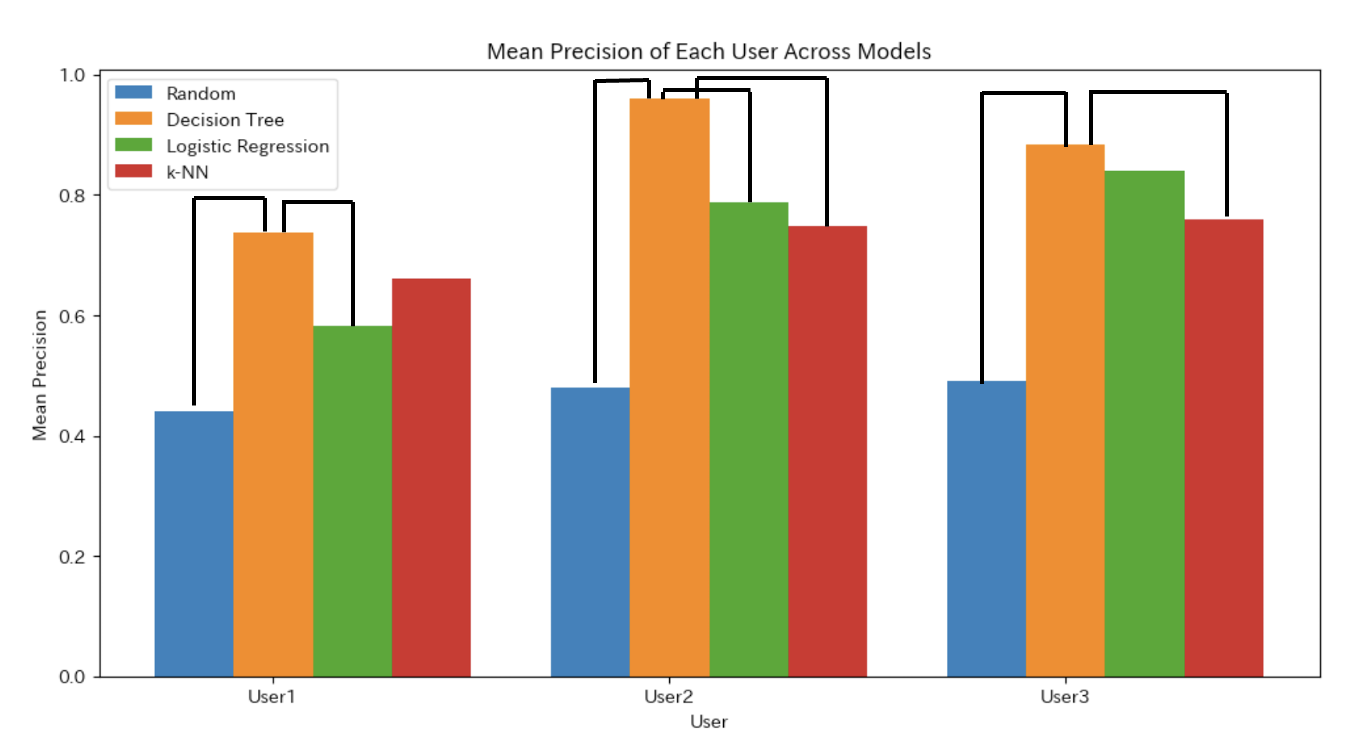
\includegraphics[width=8cm]{image/fig7.png}
      \caption{各アルゴリズムの平均精度}
      \label{fig7}
    \end{center}
\end{figure}

\subsection{訓練データを増やした際の各アルゴリズムの精度の推移}
訓練データの数を10から90に増やした際の各アルゴリズムの精度の推移を確かめた.
その結果,訓練データが少ない状況では,3つの手法はランダム手法とあまり変わらない精度であった.
訓練データが50になったところで,決定木が最も良い精度を示しており,訓練データが90の時も決定木が最も良い精度を示している.
つまり,ユーザーの評価データが十分に集まる環境であれば, 飲食店推薦には決定木を応用するのが最も良いと言える.

\section{今後の課題}
今後の課題は,写真や口コミ,位置情報といった,他にも考慮すべき特徴が存在するため,そのような特徴も考慮できるようにすることである.
\bibliographystyle{jabbrv}
\bibliography{sample}

\end{document}

